\subsubsection{Arquitectura del agente conversacional}

Este apartado presenta el estilo arquitectónico del agente, su estructura e integración, el contrato con la API del sistema, la interpretación de los mensajes, sus componentes funcionales y su integración con WhatsApp. El principio que los guía es que el NLP interpreta y el código decide.

\paragraph{Estilo arquitectónico del agente: puertos y adaptadores}

El servicio del agente sigue el estilo de puertos y adaptadores \cite{cockburn2005hexagonal} (Figura~\ref{fig:ob2_estilo_agente}). Su núcleo, el diálogo con la máquina de estados, no conoce WhatsApp, la API ni el proveedor del LLM: los usa a través de puertos, y cada tecnología se conecta con un adaptador. Así, el proveedor del LLM puede cambiarse sin modificar la conversación. El servicio no accede a la base de datos; toda operación sobre la agenda pasa por la API (RNF03).

\begin{figure}[H]
\centering
\begin{tikzpicture}[
    font=\footnotesize, >={Stealth[length=2mm]},
    adapt/.style={draw=dAgenteB, fill=white, rounded corners=3pt, line width=0.7pt, align=center, text width=2.8cm, minimum height=0.9cm, inner sep=3pt},
    ext/.style={draw=dExternoB, dashed, fill=dExternoF, rounded corners=3pt, align=center, text width=2.8cm, minimum height=0.7cm, inner sep=3pt},
    sis/.style={draw=dSistemaB, fill=dSistemaF, rounded corners=3pt, align=center, text width=2.8cm, minimum height=0.7cm, inner sep=3pt},
    fl/.style={<->, draw=black!60, line width=0.6pt}
]
    \node[regular polygon, regular polygon sides=6, minimum size=4.4cm, draw=dAgenteB, fill=dAgenteF, line width=0.8pt] (core) at (0,0) {};
    \node[align=center] at (0,0) {\textbf{Núcleo}\\[2pt] Diálogo y\\ máquina de estados\\[3pt] {\scriptsize Puertos: mensajería,}\\ {\scriptsize agenda e intérprete}};
    \node[adapt] (wa) at (-4.4,0.8) {Webhook y envío};
    \node[adapt] (rec) at (-4.4,-0.8) {Tareas programadas (recordatorios)};
    \node[adapt] (api) at (4.4,0.8) {Cliente de la API};
    \node[adapt] (nlp) at (4.4,-0.8) {Adaptador del LLM};
    \node[ext] (waX) at (-4.4,2.5) {WhatsApp (Meta)};
    \node[sis] (apiX) at (4.4,2.5) {API del sistema};
    \node[ext] (nlpX) at (4.4,-2.5) {Proveedor del LLM};
    \draw[fl] (wa.east) -- (wa.east -| core.west);
    \draw[fl] (rec.east) -- (rec.east -| core.west);
    \draw[fl] (api.west) -- (api.west -| core.east);
    \draw[fl] (nlp.west) -- (nlp.west -| core.east);
    \draw[fl] (wa) -- (waX);
    \draw[fl] (api) -- (apiX);
    \draw[fl] (nlp) -- (nlpX);
\end{tikzpicture}
\caption{Estilo de puertos y adaptadores del servicio del agente}
\label{fig:ob2_estilo_agente}
\end{figure}

\paragraph{Estructura e integración}

La Figura~\ref{fig:ob2_c4_componentes} muestra los componentes del servicio del agente y su integración con WhatsApp, el proveedor del LLM y la API del sistema. El proxy entrega el webhook al agente y bloquea desde internet la interfaz interna de la API.

\begin{figure}[H]
\centering
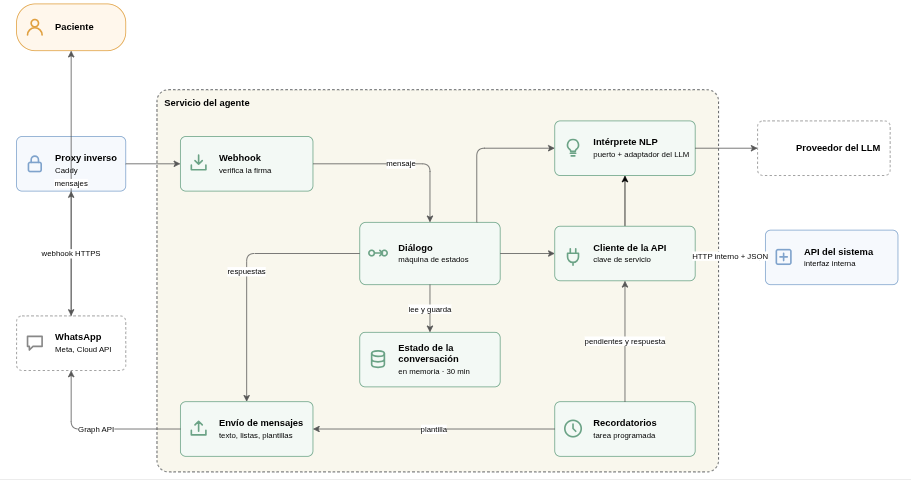
\includegraphics[width=\linewidth]{img/Objetivo2/C4_Componentes_Agente.png}
\caption{Componentes del agente y su integración (C4, nivel 3)}
\label{fig:ob2_c4_componentes}
\end{figure}

\paragraph{Contrato con la API del sistema}

El agente y la API se comunican por HTTP en la red interna del servidor, con mensajes JSON y una clave de servicio. La Tabla~\ref{tab:ob2_contrato} resume las operaciones que la API ofrece al agente. Toda operación sobre una cita recibe el teléfono, y la API comprueba que la cita le pertenezca. Las escrituras usan la misma operación de agenda que la recepción y solo se ejecutan tras la confirmación del paciente; a diferencia de \cite{shaikh2026smartmedibook}, que valida la doble reserva en la aplicación, la regla anticruce está en la base de datos y vale para ambos canales.

\begingroup
\fontsize{9}{11}\selectfont
\renewcommand{\arraystretch}{1.2}
\setlength{\LTpre}{0pt}\setlength{\LTpost}{6pt}
\setlength{\tabcolsep}{4pt}
\begin{xltabular}{\linewidth}{|>{\raggedright\arraybackslash}p{3.0cm}|>{\raggedright\arraybackslash}X|>{\raggedright\arraybackslash}p{2.0cm}|}
\caption{Contrato entre el agente y la API del sistema}
\label{tab:ob2_contrato} \\
\hline
\textbf{Grupo} & \textbf{Operaciones} & \textbf{Requerimiento} \\ \hline
\endfirsthead
\hline
\textbf{Grupo} & \textbf{Operaciones} & \textbf{Requerimiento} \\ \hline
\endhead
Aviso de privacidad & Consultar y registrar la aceptación por teléfono & RF09 \\ \hline
Información & Horarios, formas de pago, precios públicos y contacto de recepción & RF10, RF13 \\ \hline
Identificación & Pacientes del teléfono y verificación por cédula & RF11 \\ \hline
Disponibilidad & Especialidades, profesionales, días y horas libres; horarios de urgencia & RF11 \\ \hline
Citas & Citas activas; agendar, reprogramar, cancelar y confirmar & RF11, RF12 \\ \hline
Recordatorios & Pendientes de envío, resultado del envío y respuesta del paciente & RF14 \\ \hline
\multicolumn{3}{|l|}{\cellcolor{gray!10}\textbf{Respuestas que el agente distingue}} \\ \hline
Horario ocupado & Avisa y ofrece otros horarios & RF07 \\ \hline
Límite alcanzado & Explica el límite y deriva a recepción & RF11 \\ \hline
Menos de 2 h & Deriva a recepción & RF12 \\ \hline
Error o demora & Deriva a recepción & RF13 \\ \hline
\end{xltabular}
\endgroup

\paragraph{Interpretación de los mensajes}

La Figura~\ref{fig:ob2_nlp} muestra cómo se interpreta un mensaje. Los botones y las listas pasan directamente a la máquina de estados; el texto libre pasa por el LLM, que devuelve la intención y los datos del mensaje en una respuesta estructurada. Esa respuesta se valida antes de usarla, y si el modelo falla o tarda, el agente muestra el menú. El modelo recibe el texto, el paso actual y los últimos mensajes, nunca el nombre, la cédula ni el historial; no dispone de herramientas que escriban ni ve datos de otros pacientes, lo que limita el efecto de instrucciones maliciosas escritas en el mensaje.

\begin{figure}[H]
\centering
\begin{tikzpicture}[
    font=\footnotesize, >={Stealth[length=2mm]},
    paso/.style={draw=#1, rounded corners=3pt, line width=0.7pt, align=center, text width=2.1cm, minimum height=1.25cm, inner sep=3pt},
    fl/.style={->, draw=black!60, line width=0.6pt}
]
    \node[paso=dPersonaB, fill=dPersonaF] (msg) {\textbf{Mensaje}\\ del paciente};
    \node[paso=dAgenteB, fill=dAgenteF, right=0.6cm of msg] (fil) {\textbf{Filtros fijos}\\ aviso, derivación activa};
    \node[paso=dExternoB, fill=dExternoF, dashed, right=0.6cm of fil] (llm) {\textbf{LLM}\\ intención y datos};
    \node[paso=dAgenteB, fill=dAgenteF, right=0.6cm of llm] (val) {\textbf{Validación}\\ de la respuesta};
    \node[paso=dAgenteB, fill=dAgenteF, right=0.6cm of val] (fsm) {\textbf{Máquina de estados}\\ paso siguiente};
    \node[paso=dAgenteB, fill=white, below=0.9cm of val] (menu) {\textbf{Menú}};
    \draw[fl] (msg) -- (fil);
    \draw[fl] (fil) -- node[above, font=\scriptsize] {texto} (llm);
    \draw[fl] (llm) -- (val);
    \draw[fl] (val) -- (fsm);
    \draw[fl] (fil.north) -- ++(0,0.45) -| node[pos=0.25, above, font=\scriptsize] {botón o lista} (fsm.north);
    \draw[fl, dashed] (llm.south) |- node[pos=0.75, above, font=\scriptsize] {falla o demora} (menu.west);
    \draw[fl, dashed] (val) -- node[right, font=\scriptsize] {inválida} (menu);
    \draw[fl] (menu.east) -| (fsm.south);
    \end{tikzpicture}
\caption{Interpretación de un mensaje con el LLM y paso al menú ante una falla}
\label{fig:ob2_nlp}
\end{figure}

La Tabla~\ref{tab:ob2_intenciones} relaciona cada intención con la acción que decide la máquina de estados. Los precios, horarios y fechas los escribe el código con los datos de la API, nunca el modelo.

\begingroup
\fontsize{9}{11}\selectfont
\renewcommand{\arraystretch}{1.2}
\setlength{\LTpre}{0pt}\setlength{\LTpost}{6pt}
\setlength{\tabcolsep}{4pt}
\begin{xltabular}{\linewidth}{|>{\raggedright\arraybackslash}p{4.6cm}|>{\raggedright\arraybackslash}X|}
\caption{Intenciones reconocidas y acción del agente}
\label{tab:ob2_intenciones} \\
\hline
\textbf{Intención} & \textbf{Acción} \\ \hline
\endfirsthead
\hline
\textbf{Intención} & \textbf{Acción} \\ \hline
\endhead
Horarios o precios & Respuesta con los datos de la API; precio referencial \\ \hline
Agendar, reprogramar, cancelar o confirmar & Flujo de la cita con los datos extraídos; pide lo que falta \\ \hline
Dolor o urgencia & Primeros horarios de hoy o mañana y aviso de emergencia \\ \hline
Clínica, saldo o hablar con recepción & Derivación a recepción \\ \hline
Saludo o fuera de tema & Texto fijo y menú \\ \hline
No reconocida dos veces seguidas & Derivación a recepción \\ \hline
\end{xltabular}
\endgroup

\paragraph{Componentes funcionales y conversación}

La Figura~\ref{fig:ob2_componentes_func} resume los nueve componentes funcionales, el requerimiento que atiende cada uno y su regla principal. Los límites de agendamiento son configurables, los aplica la API y solo valen para el agente; la recepción no los tiene.

\begin{figure}[H]
\centering
\begin{tikzpicture}[
    tarjeta/.style 2 args={rectangle split, rectangle split parts=2, draw=#2, line width=0.7pt, rounded corners=2pt,
        rectangle split part fill={#1,white}, text width=4.3cm, align=left, inner sep=3pt, font=\scriptsize},
]
    \def\dx{4.9}
    \node[tarjeta={dAgenteF}{dAgenteB}, anchor=north] at (0,0) {\textbf{Aviso de privacidad}\nodepart{two}\textbf{RF09.} Primera interacción; sin aceptación no se tratan datos. Habilita los recordatorios.};
    \node[tarjeta={dAgenteF}{dAgenteB}, anchor=north] at (\dx,0) {\textbf{Intérprete de mensajes}\nodepart{two}\textbf{RF10, RF13.} Convierte el texto libre en intención y datos; no decide ni escribe. Si falla, se muestra el menú.};
    \node[tarjeta={dAgenteF}{dAgenteB}, anchor=north] at (2*\dx,0) {\textbf{Menú}\nodepart{two}\textbf{RF10.} Horarios, precios, agendar, reprogramar y hablar con recepción.};
    \node[tarjeta={dAgenteF}{dAgenteB}, anchor=north] at (0,-2.0) {\textbf{Identificación}\nodepart{two}\textbf{RF11.} Busca al paciente por teléfono; si hay varios, pide la cédula. Sin coincidencia, deriva.};
    \node[tarjeta={dAgenteF}{dAgenteB}, anchor=north] at (\dx,-2.0) {\textbf{Información}\nodepart{two}\textbf{RF10.} Horarios, formas de pago y precios referenciales tomados del catálogo.};
    \node[tarjeta={dAgenteF}{dAgenteB}, anchor=north] at (2*\dx,-2.0) {\textbf{Agendamiento}\nodepart{two}\textbf{RF11.} Próximos 14 días; una cita por especialidad y hasta tres por teléfono. Ante dolor, primeros horarios de hoy o mañana y aviso de emergencia, sin consejo médico.};
    \node[tarjeta={dAgenteF}{dAgenteB}, anchor=north] at (0,-4.8) {\textbf{Reprogramación}\nodepart{two}\textbf{RF12.} Hasta 2 h antes de la cita; la nueva queda enlazada con la original.};
    \node[tarjeta={dSistemaF}{dSistemaB}, anchor=north] at (\dx,-4.8) {\textbf{Recordatorios}\nodepart{two}\textbf{RF14.} El día anterior, con Confirmar, Cancelar y Reprogramar; solo datos de la cita.};
    \node[tarjeta={dPersonaF}{dPersonaB}, anchor=north] at (2*\dx,-4.8) {\textbf{Derivación}\nodepart{two}\textbf{RF13.} Consultas clínicas, de saldo o no reconocidas pasan a recepción.};
\end{tikzpicture}
\caption{Componentes funcionales del agente, con su requerimiento y regla principal}
\label{fig:ob2_componentes_func}
\end{figure}

La Figura~\ref{fig:ob2_estados_conversacion} muestra cómo se encadenan estos componentes en una conversación. El aviso solo aparece si el teléfono aún no lo aceptó, y la identificación solo se pide para agendar o reprogramar. El texto libre pasa por el intérprete antes de llegar a la máquina de estados, y los horarios y precios se responden desde el menú. El recordatorio inicia una conversación propia. El estado se guarda en memoria y caduca a los 30 min; un reinicio del servicio no pierde citas, porque una cita solo se registra al confirmarse.

\begin{figure}[H]
\centering
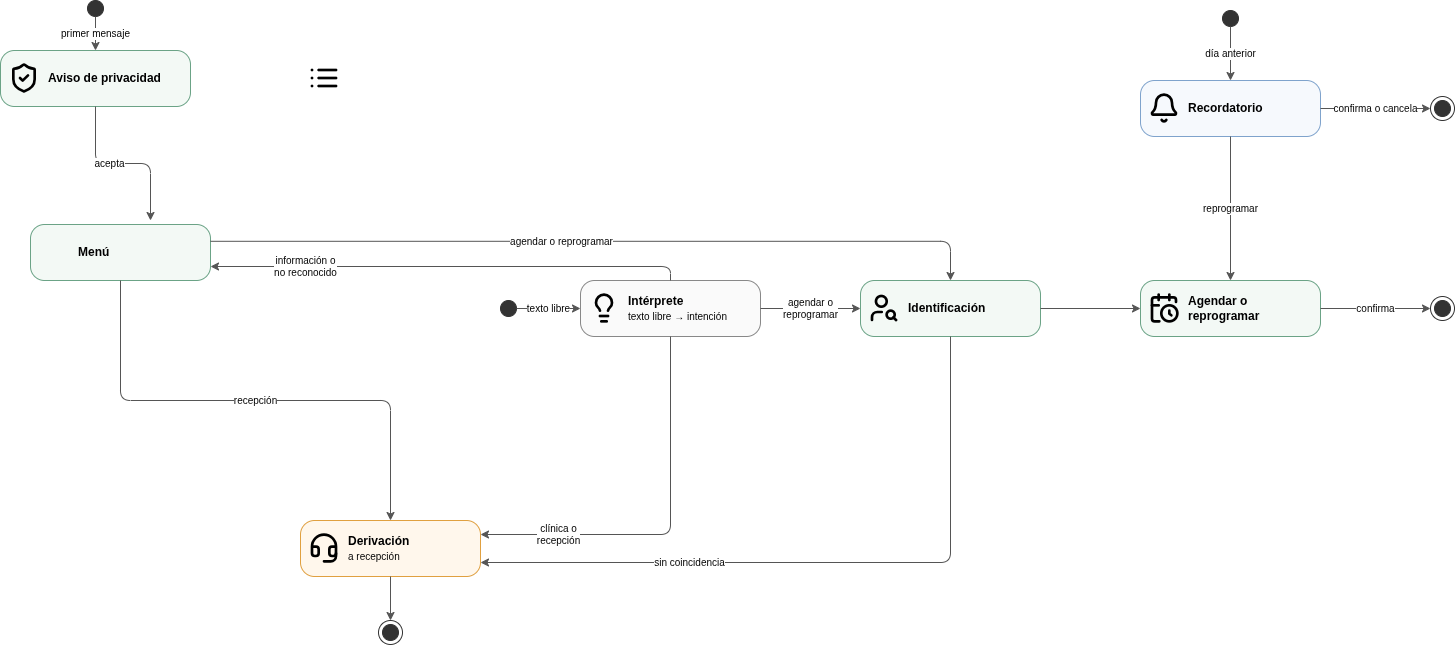
\includegraphics[width=\linewidth,height=0.85\textheight,keepaspectratio]{img/Objetivo2/Estados_Conversacion.png}
\caption{Estados de la conversación con el agente}
\label{fig:ob2_estados_conversacion}
\end{figure}
\paragraph{Integración con WhatsApp}

La Tabla~\ref{tab:ob2_mecanismos} resume los mecanismos de WhatsApp Cloud API que usa el diseño. La Figura~\ref{fig:ob2_secuencia_agendar} muestra el agendamiento a partir de un mensaje libre, y la Figura~\ref{fig:ob2_secuencia_recordatorio}, el recordatorio y su respuesta.

\begingroup
\fontsize{9}{11}\selectfont
\renewcommand{\arraystretch}{1.2}
\setlength{\LTpre}{0pt}\setlength{\LTpost}{6pt}
\setlength{\tabcolsep}{4pt}
\begin{xltabular}{\linewidth}{|>{\raggedright\arraybackslash}p{3.8cm}|>{\raggedright\arraybackslash}X|>{\raggedright\arraybackslash}p{2.2cm}|}
\caption{Mecanismos de integración con WhatsApp Cloud API}
\label{tab:ob2_mecanismos} \\
\hline
\textbf{Mecanismo} & \textbf{Uso en el diseño} & \textbf{Requerimiento} \\ \hline
\endfirsthead
\hline
\textbf{Mecanismo} & \textbf{Uso en el diseño} & \textbf{Requerimiento} \\ \hline
\endhead
Webhook verificado & Token al registrar la URL y firma en cada solicitud \cite{meta2026whatsapp} & RNF03 \\ \hline
Mensajes interactivos & Listas para el menú y la cita; botones para el recordatorio & RF10, RF11 \\ \hline
Plantillas utility & Recordatorios iniciados por la clínica, aprobados por Meta y cobrados por envío \cite{meta2026pricing} & RF14 \\ \hline
Consentimiento previo & Requisito de Meta para escribir primero \cite{meta2026optin}; se usa la aceptación del aviso & RF09, RF14 \\ \hline
Ventana de 24 h & Respuestas libres solo dentro de 24 h del último mensaje; después, plantillas & RF10, RF13 \\ \hline
Límite diario de envíos & Tope de destinatarios por día según el nivel de la cuenta \cite{meta2026limits} & RF14 \\ \hline
Enlace wa.me & Deriva al número de recepción, distinto del número del agente & RF13 \\ \hline
\end{xltabular}
\endgroup

\begin{figure}[H]
\centering
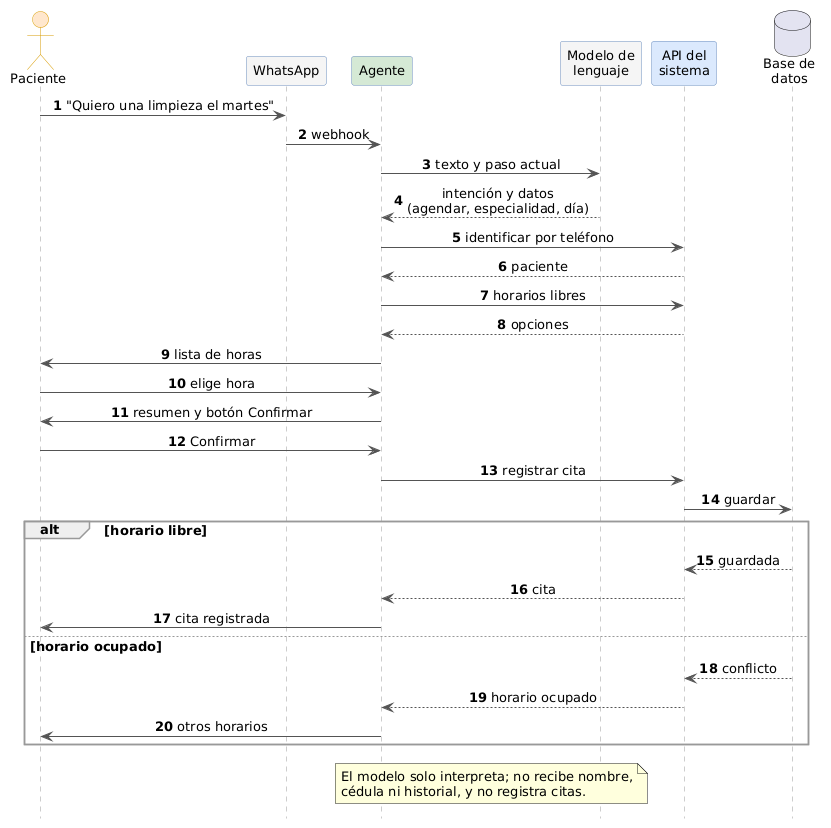
\includegraphics[width=0.85\linewidth]{img/Objetivo2/Secuencia_Agendar.png}
\caption{Agendamiento de una cita por WhatsApp, con conflicto y con éxito}
\label{fig:ob2_secuencia_agendar}
\end{figure}

\begin{figure}[H]
\centering
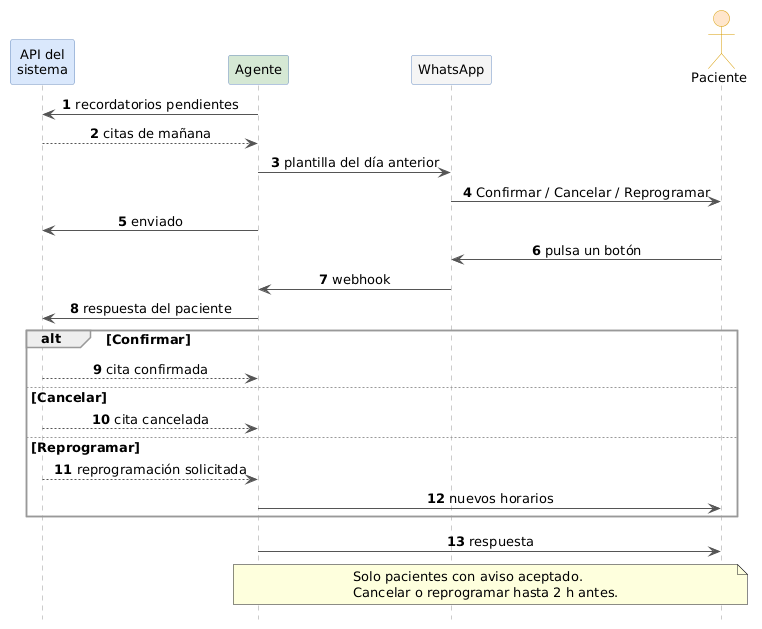
\includegraphics[width=0.85\linewidth]{img/Objetivo2/Secuencia_Recordatorio.png}
\caption{Recordatorio del día anterior y respuesta del paciente}
\label{fig:ob2_secuencia_recordatorio}
\end{figure}
